\documentclass{article}

\input{../../../latex_preambule_style/preambule}
\input{../../../latex_preambule_style/styleCoursCycle4}
\input{../../../latex_preambule_style/styleExercices}
\input{../../../latex_preambule_style/bas_de_page_quatrieme}
\input{../../../latex_preambule_style/algobox}

%%%%%%%%%%%%%%%  Indentation  %%%%%%%%%%%%%%%%%%
\parindent=0pt
%%%%%%%%%%%%%%%%%%%%%%%%%%%%%%%%%%%%%%%%%%%%%%%%
\begin{document}


\Exe

Voici un algorithme écrit avec Scratch.

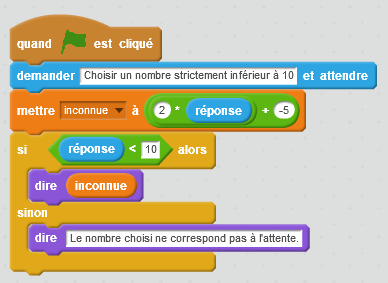
\includegraphics[scale=1]{scratch.png} 

\begin{enumerate}
\item Quelle valeur est dite si le nombre choisi est égal à 15 ?
\item Quelle valeur est dite si le nombre choisi est égal à  4 ?
\item Quelles valeurs doit-on choisir pour obtenir une valeur inférieure ou égale à 11 ? 
\item Quelles valeurs doit-on choisir pour obtenir une valeur strictement supérieure à 3 ? 
\end{enumerate}

\end{document}